\documentclass{article}
\usepackage{titlesec}
\usepackage{tikz}
\usetikzlibrary{automata,positioning}
\setcounter{secnumdepth}{4}
\titleformat{\paragraph}
{\normalfont\normalsize\bfseries}{\theparagraph}{1em}{}
\titlespacing*{\paragraph}
{0pt}{3.25ex plus 1ex minus .2ex}{1.5ex plus .2ex}

\begin{document}
\section{Automatas:}
\subsection{Accept words starting with two consecutive a's:}
$A = (\{q_0, q_a, q_{aa}, q_{fail}\}, \{a, b\}, \delta, {q_{aa}})$ \newline
\begin{tikzpicture}[shorten >=1pt,node distance=4cm,on grid,auto] 
   \node[state,initial] (q_0)   {$q_0$}; 
   \node[state] (q_a) [above right=of q_0] {$q_a$}; 
   \node[state] (q_{fail}) [below right=of q_0] {$q_{fail}$}; 
   \node[state,accepting](q_{aa}) [below right=of q_a] {$q_{aa}$};
    \path[->] 
    (q_0) edge node {a} (q_a)
          edge node {b} (q_{fail})
    (q_a) edge node {a} (q_{aa})
          edge node {b} (q_{fail})
    (q_{aa}) edge [loop below] node {{a,b}} () 
    (q_{fail}) edge [loop below] node {{a,b}} ();
\end{tikzpicture}
\newline
\subsection{Accept no words:}
$A = (\{q_0\}, \{a,b\}, \delta, \emptyset)$ \newline
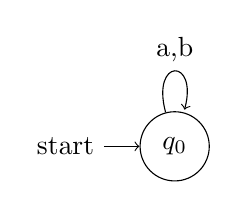
\begin{tikzpicture}
  \node [state, initial] (q_0) {$q_0$};
    \path[->]
    (q_0) edge [loop above] node {{a,b}} ();
\end{tikzpicture}

\subsection{Accept all words:}
$A = (\{q_0\}, \{a,b\}, \delta, \Sigma^{*})$ \newline
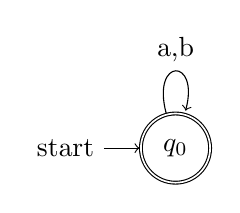
\begin{tikzpicture}
  \node [state, initial, accepting] (q_0) {$q_0$};
    \path[->]
    (q_0) edge [loop above] node {{a,b}} ();
\end{tikzpicture}
\subsection{Only accept empty words ($\epsilon$):}
$A = (\{q_0, q_{fail}\}, \{a,b\}, \delta, \{\epsilon\})$ \newline
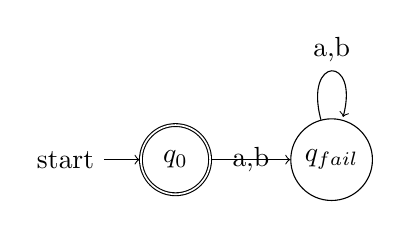
\begin{tikzpicture}
  \node [state, initial, accepting] (q_0) {$q_0$};
  \node [state] (q_{fail}) [right=of q_0]{$q_{fail}$};
  
    \path[->]
    (q_0) edge node {{a,b}} (q_{fail})
    (q_{fail}) edge [loop above] node {{a,b}} ();
\end{tikzpicture}
\subsection{Only accept words which have their odd characters set to a:}
$A = (\{q_{even}, q_{odd}, q_{fail}\}, \{a,b\}, \delta, \{\exists x \in \Sigma^{*} \exists y,z \in \Sigma \mid x = yz \wedge z = a\})$ \newline
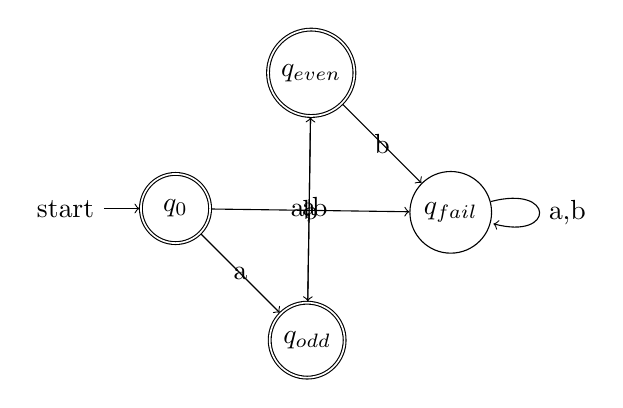
\begin{tikzpicture}
  \node [state, initial, accepting] (q_0) {$q_0$};
  \node [state, accepting] (q_{even}) [above right=of q_0] {$q_{even}$};
  \node [state, accepting] (q_{odd}) [below right=of q_0] {$q_{odd}$};
  \node [state] (q_{fail}) [below right=of q_{even}] {$q_{fail}$};
    \path[->]
    (q_0) edge node {a} (q_{odd})
    (q_0) edge node {b} (q_{fail})
    (q_{even}) edge node {a} (q_{odd})
    (q_{even}) edge node {b} (q_{fail})
    (q_{odd}) edge node {{a,b}} (q_{even})
    (q_{fail}) edge [loop right] node {{a,b}} (q_{fail});
\end{tikzpicture}
\subsection{Only accept words which have their first character set differently than the last:}
$A = (\{q_{even}, q_{odd}, q_{fail}\}, \{a,b\}, \delta, \{x = wyz \mid w,z \in \Sigma \wedge y \in \Sigma^{*} \wedge w \neq z\})$ \newline
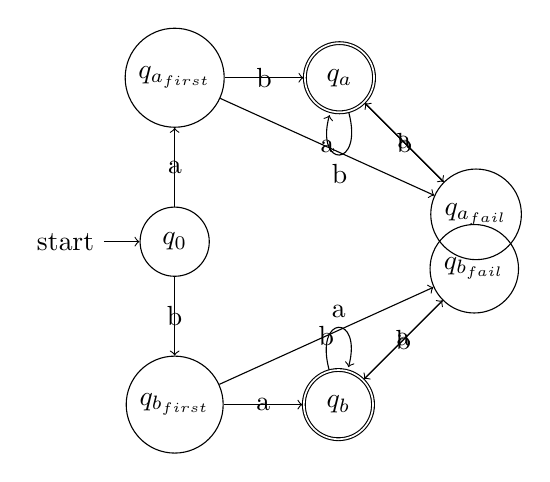
\begin{tikzpicture}
  \node [state, initial] (q_0) {$q_0$};
  \node [state] (q_{a_{first}}) [above=of q_0]{$q_{a_{first}}$};
  \node [state] (q_{b_{first}}) [below=of q_0]{$q_{b_{first}}$};
  \node [state, accepting] (q_a) [right=of q_{a_{first}}] {$q_a$};
  \node [state, accepting] (q_b) [right=of q_{b_{first}}] {$q_b$};
  \node [state] (q_{a_{fail}}) [below right=of q_a] {$q_{a_{fail}}$};
  \node [state] (q_{b_{fail}}) [above right=of q_b] {$q_{b_{fail}}$};
    \path[->]
    (q_0) edge node {a} (q_{a_{first}})
    (q_0) edge node {b} (q_{b_{first}})
    (q_{a_{first}}) edge node {a} (q_{a_{fail}})
    (q_{a_{first}}) edge node {b} (q_a)
    (q_{b_{first}}) edge node {b} (q_{b_{fail}})
    (q_{b_{first}}) edge node {a} (q_b)
    (q_a) edge node {a} (q_{a_{fail}})
    (q_a) edge [loop below] node {b} ()
    (q_b) edge node {b} (q_{b_{fail}})
    (q_b) edge [loop above] node {a} ()
    (q_{a_{fail}}) edge node {b} (q_a)
    (q_{b_{fail}}) edge node {a} (q_b);
\end{tikzpicture}
\subsection{Only accept words which contain the string aba:}
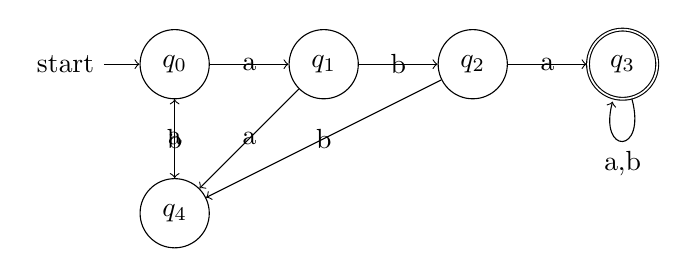
\begin{tikzpicture}
  \node [state, initial] (q_0) {$q_0$};
  \node [state] (q_1) [right=of q_0] {$q_1$};
  \node [state] (q_2) [right=of q_1] {$q_2$};
  \node [state, accepting] (q_3) [right=of q_2] {$q_3$};
  \node [state] (q_4) [below=of q_0] {$q_4$};
    \path[->]
    (q_0) edge node {a} (q_1)
    (q_0) edge node {b} (q_4)
    (q_1) edge node {b} (q_2)
    (q_1) edge node {a} (q_4)
    (q_2) edge node {b} (q_4)
    (q_2) edge node {a} (q_3)
    (q_3) edge [loop below] node {{a,b}} ()
    (q_4) edge node {a} (q_0);
\end{tikzpicture}
\subsection{Only accept words which do not contain the string aba:}
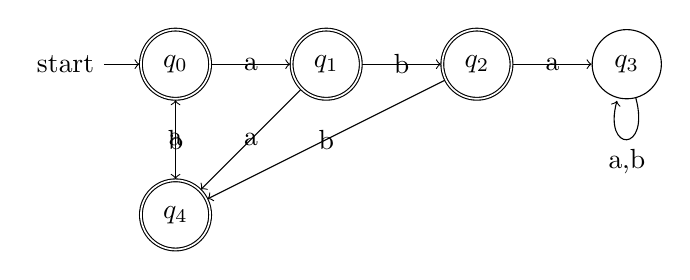
\begin{tikzpicture}
  \node [state, initial, accepting] (q_0) {$q_0$};
  \node [state, accepting] (q_1) [right=of q_0] {$q_1$};
  \node [state, accepting] (q_2) [right=of q_1] {$q_2$};
  \node [state] (q_3) [right=of q_2] {$q_3$};
  \node [state, accepting] (q_4) [below=of q_0] {$q_4$};
    \path[->]
    (q_0) edge node {a} (q_1)
    (q_0) edge node {b} (q_4)
    (q_1) edge node {b} (q_2)
    (q_1) edge node {a} (q_4)
    (q_2) edge node {b} (q_4)
    (q_2) edge node {a} (q_3)
    (q_3) edge [loop below] node {{a,b}} ()
    (q_4) edge node {a} (q_0);
\end{tikzpicture}
\subsection{Only accept words are numbers divisible by 3:}
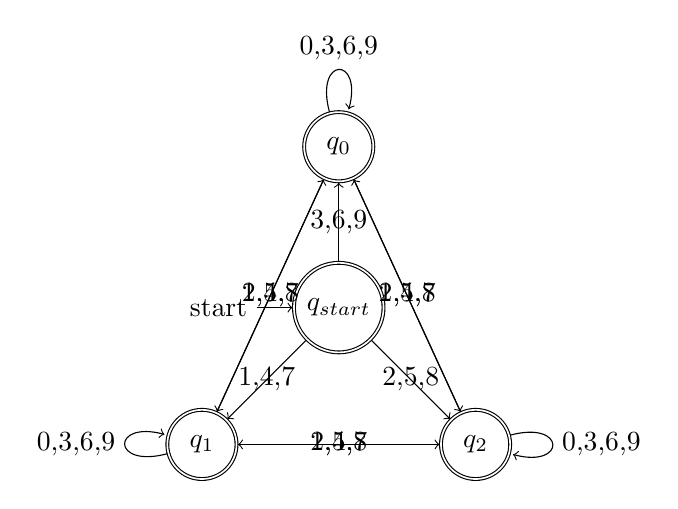
\begin{tikzpicture}
  \node [state, initial, accepting] (q_{start}) {$q_{start}$};
  \node [state, accepting] [above=of q_{start}] (q_0) {$q_0$};
  \node [state, accepting] (q_1) [below left=of q_{start}] {$q_1$};
  \node [state, accepting] (q_2) [below right=of q_{start}] {$q_2$};
    \path[->]
    (q_{start}) edge node {{1,4,7}} (q_1)
    (q_{start}) edge node {{2,5,8}} (q_2)
    (q_{start}) edge node {{3,6,9}} (q_0)
    (q_0) edge node {{1,4,7}} (q_1)
    (q_0) edge node {{2,5,8}} (q_2)
    (q_0) edge [loop above] node {{0,3,6,9}} ()
    (q_1) edge node {{1,4,7}} (q_2)
    (q_1) edge node {{2,5,8}} (q_0)
    (q_1) edge [loop left] node {{0,3,6,9}} ()
    (q_2) edge node {{1,4,7}} (q_0)
    (q_2) edge node {{2,5,8}} (q_1)
    (q_2) edge [loop right] node {{0,3,6,9}} ();
\end{tikzpicture}
\end{document}  
